% \documentclass{beamer}
% \usetheme{Szeged}

% \usepackage{media9}
% \usepackage{graphicx}

% \begin{document}

%-------------------------------------------------------------------------------
%							THIRD SECTION
%-------------------------------------------------------------------------------
\section{Le problème en 1D}

\subsection{Simulation}

\begin{frame}[fragile]
    \frametitle{Exemple de simulation 1D}
  \begin{center}
    \includemedia[
      width=0.95\linewidth,
      activate=pageopen,
      addresource=Video1D.mp4,
      flashvars={
         source=Video1D.mp4
        &autoPlay=true
      },
      passcontext, % enable VPlayer's right-click menue
    ]{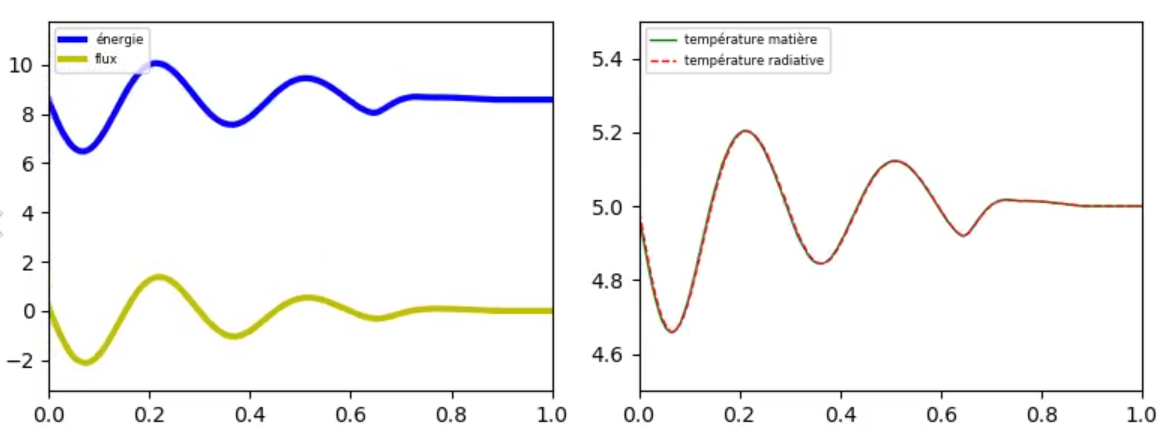
\includegraphics{Thumbnail1D.png}}{VPlayer.swf}%
  \end{center}
\end{frame}

\begin{frame}[fragile]
    \frametitle{Entrées/sorties 1D}

    \begin{columns}
    \begin{column}{0.7\textwidth}
        \begin{figure}
        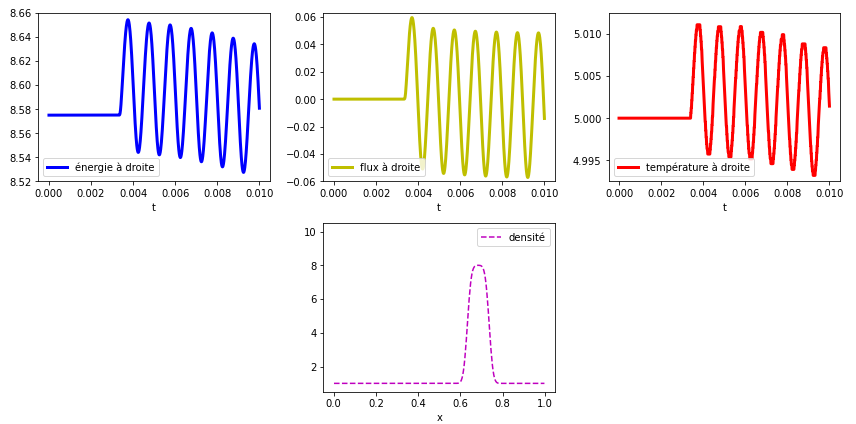
\includegraphics[width=8cm]{EntreeSortie1D}       
        \caption{Une entrée du réseau de neurones et la sortie attendue}
        \end{figure}
     \end{column}
     \begin{column}{0.3\textwidth}
        \begin{figure}
        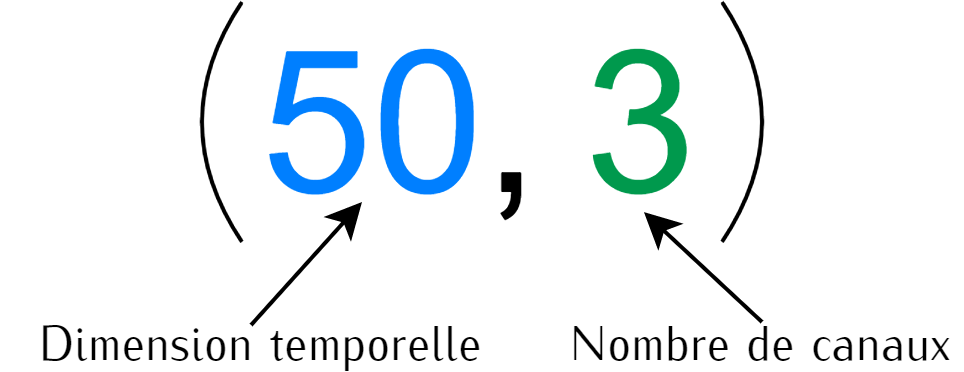
\includegraphics[width=3cm]{Entrees1D}       
        \caption{Taille d'une entrée}
        \end{figure}
     \end{column}
    \end{columns}

\end{frame}

\subsection{Apprentissage}

\begin{frame}[fragile]
    \frametitle{Meilleures/pires prédictions du CNN}

    \begin{columns}
    \begin{column}{0.5\textwidth}
        \begin{figure}
        \includegraphics<1->[width=4cm]{Meilleur1D2}       
        \includegraphics<1->[width=4cm]{Meilleur1D1}       
        \only<1->{\caption{Les meilleures prédictions}}
        \end{figure}
     \end{column}
     \begin{column}{0.5\textwidth}
        \begin{figure}
        \includegraphics<2>[width=4cm]{Pire1D1}       
        \includegraphics<2>[width=4cm]{Pire1D2}       
        \only<2>{\caption{Les pires prédictions}}
        \end{figure}
     \end{column}
    \end{columns}

\end{frame}

\begin{frame}
    \frametitle{Les scores obtenus en 1D}

    \begin{table}[h!]
        \centering
        \begin{tabular}{l l}
        \toprule
        \textbf{Nom du score} & \textbf{Valeur} \\
        \midrule
        R2 & 99.50 \%\\
        Personnalisé & 28.21 \%\\
        \bottomrule\\
        \end{tabular}
    \end{table}

    \begin{columns}
        \begin{column}{0.5\textwidth}
            \begin{figure}
            \includegraphics<2->[width=2cm]{Position1D}       
            \only<2->{\caption{Correlation des positions}}
            \end{figure}
         \end{column}
         \begin{column}{0.5\textwidth}
            \begin{figure}
            \includegraphics<3>[width=2cm]{Hauteur1D}       
            \only<3>{\caption{Correlation des hauteurs}}
            \end{figure}
         \end{column}
    \end{columns}

\end{frame}


\begin{frame}[fragile]
    \frametitle{Conclusion sur la régression 1D}
Les cause de l'échec :
\pause
\begin{itemize}
    \item Le problème inverse est probablement mal posé  % EN supposant que je n'ai commise aucune erreur
    \item Le score R2 est mal calculé % Non prise en compte des poinds 10:1. 
\end{itemize}
\scriptsize

\begin{verbatim}
    from keras import backend as K
    
     def r2_score(y_true, y_pred):
        SS_res =  K.sum(K.square(y_true - y_pred), axis=-1) 
        SS_tot = K.sum(K.square(y_true - K.mean(y_true)), axis=-1)
        return 1.0 - SS_res/(SS_tot + K.epsilon())
\end{verbatim}

\end{frame}


% \end{document}
